\documentclass[10pt,a4paper,spanish]{article}

\usepackage[spanish]{babel}
\usepackage[utf8]{inputenc}
\usepackage{amsmath, amsthm}
\usepackage{amsfonts, amssymb, latexsym}
\usepackage{enumerate}
% \usepackage[official]{eurosym}
\usepackage{graphicx}
\usepackage[usenames, dvipsnames]{color}
\usepackage{colortbl}
\usepackage{multirow}
\usepackage{fancyhdr}
\usepackage[all]{xy}
% \usepackage{minted}
\usepackage{float}
\usepackage{subfigure}
\usepackage{tikz}
\usepackage{pgfplots}
\usepackage{cancel}
\pgfplotsset{compat=1.5}

\usepackage[top=2.5cm, bottom=2.5cm, left=3cm, right=3cm]{geometry}

\usepackage[bookmarks=true,
            bookmarksnumbered=false, % true means bookmarks in
                                     % left window are numbered
            bookmarksopen=false,     % true means only level 1
                                     % are displayed.
            colorlinks=true,
            linkcolor=red,
            citecolor=blue]{hyperref}

\newcommand{\HRule}{\rule{\linewidth}{0.5mm}} % regla horizontal para  el titulo

\pagestyle{plain}
%con esto nos aseguramos de que las cabeceras de capítulo y de sección vayan en minúsculas

\fancyhf{} %borra cabecera y pie actuales
% \fancyhead[LE,RO]{}
% \fancyhead[LO]{}
\fancyfoot[C]{\thepage}
% \renewcommand{\headrulewidth}{0.5pt}
% \renewcommand{\footrulewidth}{0pt}
% \addtolength{\headheight}{0.5pt} %espacio para la raya
% \fancypagestyle{plain}{%
%       \fancyhead{} %elimina cabeceras en páginas "plain"
%       \renewcommand{\headrulewidth}{0pt} %así como la raya
% }

% %%%%% Para cambiar el tipo de letra en el título de la sección %%%%%%%%%%%
% \usepackage{sectsty}
% \chapterfont{\fontfamily{frc}\selectfont}
% \sectionfont{\fontfamily{pag}\selectfont}
% \subsectionfont{\fontfamily{pag}\selectfont}
% \subsubsectionfont{\fontfamily{pag}\selectfont}

% \newmintedfile[mycplusplus]{c++}{
%     linenos,
%     numbersep=5pt,
%     gobble=0,
%     frame=lines,
%     framesep=2mm,
%     tabsize=3,
% }

% \newmintedfile[mypython]{python}{
%     linenos,
%     numbersep=5pt,
%     gobble=0,
%     frame=lines,
%     framesep=2mm,
%     tabsize=3,
% }

\definecolor{amaranth}{rgb}{0.9, 0.17, 0.31}

\usepackage{arev}
\usepackage[T1]{fontenc}

\setlength{\parindent}{0pt}
\setlength{\parskip}{1ex plus 0.5ex minus 0.2ex}

% \usepackage{titlesec}

% % \titleformat{\chapter}{\normalfont\huge\center}{--- \thechapter ---}{20pt}{}

% \titleformat
% {\chapter} % command
% [display] % shape
% {\Huge\center\bfseries} % format
% {--- \thechapter ---} % label
% {0.5ex} % sep
% {
%     \rule{\textwidth}{1pt}
%     \vspace{1ex}
%     \centering
% } % before-code
% [
% \vspace{-0.5ex}%
% \rule{\textwidth}{0.3pt}
% ] % after-code

%Definimos autor y título
\title{\Huge Arquitectura de las Redes \textit{Tor}}
\author{\Large Marta Gómez Macías y Braulio Vargas López}

\begin{document}
\renewcommand{\tablename}{Tabla}
\maketitle

\section{¿Qué es \textit{Tor}?}
Según \cite{deftor}, ``la red Tor es un grupo de servidores operativos voluntarios que permiten a las personas mejorar su privacidad y seguridad en Internet''. Esto quiere decir que una conexión a través de Tor nunca será directa, sino que pasará por estos servidores voluntarios para que no se pueda saber quién manda el paquete ni a dónde va dirigido. Además, Tor también se define como ``una efectiva herramienta para la elusión de la censura, permitiendo a sus usuarios acceder a contenido que de otra forma se encontraría bloqueado.''

\subsection{¿Por qué es \textit{Tor} protege mejor la privacidad que otras herramientas?}
Tal y como se explica en \cite{deftor}, usando Tor nos protegemos contra el ``análisis de tráfico''. Aunque el \textit{payload} de los paquetes que enviamos a través de la red se encuentre encriptado, la cabecera normalmente no suele estarlo ya que se necesita para dirigir el paquete. Ésta cabecera facilita a los ``sniffers'' muchísima información sobre lo que estamos haciendo ya que incluye información como el ``host'' emisor, el ``host'' destino, el tamaño, el puerto al que va dirigido, etc.

Así, tal y como se indica en \cite{protectionstor}, Tor defiende la privacidad en tres sentidos:
\begin{enumerate}[$\bullet$]
    \item Evita que servicios tales como páginas webs (entre otros) sepan nuestra localización, la cual pueden usar para hacer una base de datos sobre nuestras costumbres e intereses. Con \textit{Tor} podemos elegir qué información compartimos y cuál no.
    \item Evita el análisis de nuestro tráfico (que, por ejemplo, puede hacer nuestro proveedor de internet) viendo la información que compartimos y desde dónde. Y también nos permite acceder a sitios web bloqueados.
    \item Tor dirige nuestra conexión por más de un \textit{relay}\footnote{Un \textit{relay} se refiere a cada servidor por el cual se envían nuestros paquetes.}, por lo que ningún \textit{relay} puede saber lo que hacemos. Esta arquitectura de \textit{relays} distribuidos (y que pertenecen a distintas personas/organizaciones) da mayor privacidad.
\end{enumerate}

Ahora bien, tal y como se aclara en \cite{anonymoustor}, usar Tor no es sinónimo de ser completamente anónimo en internet, pues lo único que protege Tor es la ruta de los paquetes que enviamos y no su contenido. Por lo que si, por ejemplo, nos conectamos a \textit{Facebook} desde Tor, \textit{Facebook} no sabrá desde dónde nos estamos conectando pero sí que sabrá nuestra identidad.

\section{¿Cómo mantiene \textit{Tor} el anonimato?}

El anonimato en \textit{Tor} se mantiene distribuyendo los paquetes que enviamos y recibimos por una gran cantidad de puntos distribuidos por internet, antes de llegar al destino, en vez de hacer una conexión directa entre el origen y el destino. Los paquetes de datos seguirán un camino aleatorio entre los distintos ``relevos'' que existen en la red de Tor, que eliminan nuestras $huellas$, para que en ningún punto del camino que toma el paquete se pueda saber de dónde viene el paquete y a dónde va.

Para crear un camino en la red privada de Tor, se crea un circuito incremental de conexiones encriptadas a través de los ``relevos'' de la red, como podemos ver en la \hyperref[htw1]{Figura \ref*{htw1}}. Los incrementos del circuito se hacen de uno en uno cada vez, y cada punto del circuito sólo sabe de qué relevo viene el paquete, y a qué relevo se lo tiene que dar. El cliente aporta un conjunto de llaves diferentes para encriptar el mensaje para cada punto del circuito para asegurarse de que en cada punto del circuito no se pueda seguir el paquete (\hyperref[htw2]{Figura \ref*{htw2}}). Gracias a esto, como un nodo solo conoce de qué nodo viene la información y a qué nodo tiene que mandarla, 

Por eficiencia, el mismo circuito tiene una vida de 10 minutos más o menos. Para las siguientes conexiones obtienen un nuevo circuito, como se ve en la \hyperref[htw3]{Figura \ref*{htw3}}.

\begin{figure}[H]
    \centering
    
    \mbox {
        \subfigure[Inicio de la conexión Tor. Al inicio de la conexión obtenemos una lista de nodos Tor del directorio del servidor.]{
            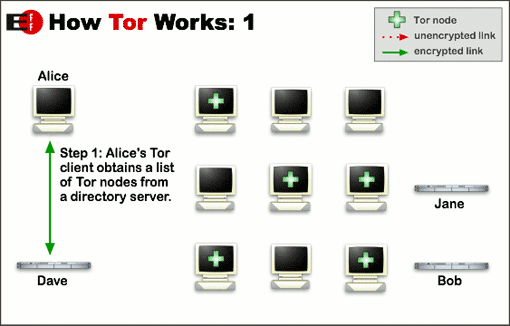
\includegraphics[width=0.5\textwidth]{htw1}
            \label{htw1}
        }
        
        \qquad
    
        \subfigure[Circuito o camino creado para la conexión. Como se ve en la imagen, los enlaces en verde están encriptados y los rojos no.] {
            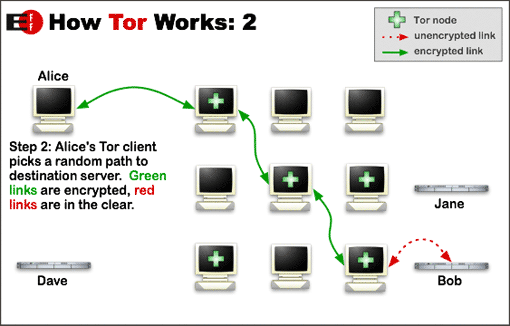
\includegraphics[width=0.51\textwidth]{htw2}
            \label{htw2}
        }
    }

    \mbox{
        \subfigure[Si se realiza una conexión más allá de esos 10 minutos, se genera un nuevo circuito.] {
            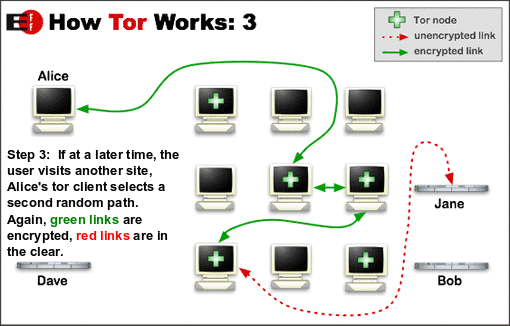
\includegraphics[width=0.51\textwidth]{htw3}
            \label{htw3}
        }
    }
    \caption{Cómo funciona Tor.}
    \label{htw}
\end{figure} 

\section{Arquitectura}
En la sección ``The Tor Design'' de \cite{design}, encontramos una descripción detallada de la arquitectura de \textit{Tor}. Un paquete Tor tiene exactamente 512 bytes y está compuesto por una cabecera y un payload. 

En la \hyperref[paquete]{Figura \ref*{paquete}} vemos una representación gráfica de un paquete Tor. La cabecera incluye tanto el identificador del circuito (que indica a qué circuito pertenece el paquete) como un comando que describe qué hacer con el payload. Según sea dicho comando, los paquetes pueden ser tanto de \textbf{control} como de \textbf{relay}. Un paquete de control debe ser interpretado por el nodo que lo recibe y sirve para operar con el circuito y uno de relay, sólo contiene datos.

Los paquetes \textit{relay} tienen una cabecera adicional antes del payload. Ésta cabecera contiene el \textit{streamID}, un \textit{checksum} para poder hacer una comprobación de integridad, la longitud del payload y un comando \textit{relay}, que puede tomar valores para operar tanto con el stream de datos como con el circuito y para hacer un control de congestión.

\begin{figure}[!h]
    \centering
    % Graphic for TeX using PGF
% Title: /home/marta/Documentos/Git/Arquitectura-Redes-Tor/PDFResumen/Diagrama1.dia
% Creator: Dia v0.97.3
% CreationDate: Tue Dec  8 21:22:44 2015
% For: marta
% \usepackage{tikz}
% The following commands are not supported in PSTricks at present
% We define them conditionally, so when they are implemented,
% this pgf file will use them.
\ifx\du\undefined
  \newlength{\du}
\fi
\setlength{\du}{15\unitlength}
\begin{tikzpicture}
\pgftransformxscale{1.000000}
\pgftransformyscale{-1.000000}
\definecolor{dialinecolor}{rgb}{0.000000, 0.000000, 0.000000}
\pgfsetstrokecolor{dialinecolor}
\definecolor{dialinecolor}{rgb}{1.000000, 1.000000, 1.000000}
\pgfsetfillcolor{dialinecolor}
\definecolor{dialinecolor}{rgb}{1.000000, 1.000000, 1.000000}
\pgfsetfillcolor{dialinecolor}
\fill (5.100000\du,5.000000\du)--(5.100000\du,6.900000\du)--(10.050000\du,6.900000\du)--(10.050000\du,5.000000\du)--cycle;
\pgfsetlinewidth{0.100000\du}
\pgfsetdash{}{0pt}
\pgfsetdash{}{0pt}
\pgfsetmiterjoin
\definecolor{dialinecolor}{rgb}{0.000000, 0.000000, 0.000000}
\pgfsetstrokecolor{dialinecolor}
\draw (5.100000\du,5.000000\du)--(5.100000\du,6.900000\du)--(10.050000\du,6.900000\du)--(10.050000\du,5.000000\du)--cycle;
% setfont left to latex
\definecolor{dialinecolor}{rgb}{0.000000, 0.000000, 0.000000}
\pgfsetstrokecolor{dialinecolor}
\node at (7.575000\du,6.145000\du){CircID};
% setfont left to latex
\definecolor{dialinecolor}{rgb}{0.000000, 0.000000, 0.000000}
\pgfsetstrokecolor{dialinecolor}
\node[anchor=west] at (7.450000\du,4.500000\du){2};
\definecolor{dialinecolor}{rgb}{1.000000, 1.000000, 1.000000}
\pgfsetfillcolor{dialinecolor}
\fill (10.053750\du,5.000000\du)--(10.053750\du,6.900000\du)--(12.646250\du,6.900000\du)--(12.646250\du,5.000000\du)--cycle;
\pgfsetlinewidth{0.100000\du}
\pgfsetdash{}{0pt}
\pgfsetdash{}{0pt}
\pgfsetmiterjoin
\definecolor{dialinecolor}{rgb}{0.000000, 0.000000, 0.000000}
\pgfsetstrokecolor{dialinecolor}
\draw (10.053750\du,5.000000\du)--(10.053750\du,6.900000\du)--(12.646250\du,6.900000\du)--(12.646250\du,5.000000\du)--cycle;
% setfont left to latex
\definecolor{dialinecolor}{rgb}{0.000000, 0.000000, 0.000000}
\pgfsetstrokecolor{dialinecolor}
\node at (11.350000\du,6.145000\du){CMD};
% setfont left to latex
\definecolor{dialinecolor}{rgb}{0.000000, 0.000000, 0.000000}
\pgfsetstrokecolor{dialinecolor}
\node[anchor=west] at (11.300000\du,4.350000\du){1};
\definecolor{dialinecolor}{rgb}{1.000000, 1.000000, 1.000000}
\pgfsetfillcolor{dialinecolor}
\fill (12.700000\du,5.000000\du)--(12.700000\du,6.900000\du)--(26.950000\du,6.900000\du)--(26.950000\du,5.000000\du)--cycle;
\pgfsetlinewidth{0.100000\du}
\pgfsetdash{}{0pt}
\pgfsetdash{}{0pt}
\pgfsetmiterjoin
\definecolor{dialinecolor}{rgb}{0.000000, 0.000000, 0.000000}
\pgfsetstrokecolor{dialinecolor}
\draw (12.700000\du,5.000000\du)--(12.700000\du,6.900000\du)--(26.950000\du,6.900000\du)--(26.950000\du,5.000000\du)--cycle;
% setfont left to latex
\definecolor{dialinecolor}{rgb}{0.000000, 0.000000, 0.000000}
\pgfsetstrokecolor{dialinecolor}
\node at (19.825000\du,6.145000\du){DATA};
% setfont left to latex
\definecolor{dialinecolor}{rgb}{0.000000, 0.000000, 0.000000}
\pgfsetstrokecolor{dialinecolor}
\node[anchor=west] at (18.100000\du,4.600000\du){509  bytes};
\definecolor{dialinecolor}{rgb}{1.000000, 1.000000, 1.000000}
\pgfsetfillcolor{dialinecolor}
\fill (4.996250\du,8.100000\du)--(4.996250\du,10.000000\du)--(8.003750\du,10.000000\du)--(8.003750\du,8.100000\du)--cycle;
\pgfsetlinewidth{0.100000\du}
\pgfsetdash{}{0pt}
\pgfsetdash{}{0pt}
\pgfsetmiterjoin
\definecolor{dialinecolor}{rgb}{0.000000, 0.000000, 0.000000}
\pgfsetstrokecolor{dialinecolor}
\draw (4.996250\du,8.100000\du)--(4.996250\du,10.000000\du)--(8.003750\du,10.000000\du)--(8.003750\du,8.100000\du)--cycle;
% setfont left to latex
\definecolor{dialinecolor}{rgb}{0.000000, 0.000000, 0.000000}
\pgfsetstrokecolor{dialinecolor}
\node at (6.500000\du,9.245000\du){CircID};
% setfont left to latex
\definecolor{dialinecolor}{rgb}{0.000000, 0.000000, 0.000000}
\pgfsetstrokecolor{dialinecolor}
\node[anchor=west] at (6.363388\du,7.712500\du){2};
\definecolor{dialinecolor}{rgb}{1.000000, 1.000000, 1.000000}
\pgfsetfillcolor{dialinecolor}
\fill (7.968750\du,8.100000\du)--(7.968750\du,10.000000\du)--(10.831250\du,10.000000\du)--(10.831250\du,8.100000\du)--cycle;
\pgfsetlinewidth{0.100000\du}
\pgfsetdash{}{0pt}
\pgfsetdash{}{0pt}
\pgfsetmiterjoin
\definecolor{dialinecolor}{rgb}{0.000000, 0.000000, 0.000000}
\pgfsetstrokecolor{dialinecolor}
\draw (7.968750\du,8.100000\du)--(7.968750\du,10.000000\du)--(10.831250\du,10.000000\du)--(10.831250\du,8.100000\du)--cycle;
% setfont left to latex
\definecolor{dialinecolor}{rgb}{0.000000, 0.000000, 0.000000}
\pgfsetstrokecolor{dialinecolor}
\node at (9.400000\du,9.245000\du){Relay};
% setfont left to latex
\definecolor{dialinecolor}{rgb}{0.000000, 0.000000, 0.000000}
\pgfsetstrokecolor{dialinecolor}
\node[anchor=west] at (9.313020\du,7.688388\du){1};
\definecolor{dialinecolor}{rgb}{1.000000, 1.000000, 1.000000}
\pgfsetfillcolor{dialinecolor}
\fill (10.801250\du,8.100000\du)--(10.801250\du,10.000000\du)--(14.898750\du,10.000000\du)--(14.898750\du,8.100000\du)--cycle;
\pgfsetlinewidth{0.100000\du}
\pgfsetdash{}{0pt}
\pgfsetdash{}{0pt}
\pgfsetmiterjoin
\definecolor{dialinecolor}{rgb}{0.000000, 0.000000, 0.000000}
\pgfsetstrokecolor{dialinecolor}
\draw (10.801250\du,8.100000\du)--(10.801250\du,10.000000\du)--(14.898750\du,10.000000\du)--(14.898750\du,8.100000\du)--cycle;
% setfont left to latex
\definecolor{dialinecolor}{rgb}{0.000000, 0.000000, 0.000000}
\pgfsetstrokecolor{dialinecolor}
\node at (12.850000\du,9.245000\du){StreamID};
% setfont left to latex
\definecolor{dialinecolor}{rgb}{0.000000, 0.000000, 0.000000}
\pgfsetstrokecolor{dialinecolor}
\node[anchor=west] at (12.557322\du,7.658211\du){2};
\definecolor{dialinecolor}{rgb}{1.000000, 1.000000, 1.000000}
\pgfsetfillcolor{dialinecolor}
\fill (14.922500\du,8.100000\du)--(14.922500\du,10.000000\du)--(18.077500\du,10.000000\du)--(18.077500\du,8.100000\du)--cycle;
\pgfsetlinewidth{0.100000\du}
\pgfsetdash{}{0pt}
\pgfsetdash{}{0pt}
\pgfsetmiterjoin
\definecolor{dialinecolor}{rgb}{0.000000, 0.000000, 0.000000}
\pgfsetstrokecolor{dialinecolor}
\draw (14.922500\du,8.100000\du)--(14.922500\du,10.000000\du)--(18.077500\du,10.000000\du)--(18.077500\du,8.100000\du)--cycle;
% setfont left to latex
\definecolor{dialinecolor}{rgb}{0.000000, 0.000000, 0.000000}
\pgfsetstrokecolor{dialinecolor}
\node at (16.500000\du,9.245000\du){Digest};
% setfont left to latex
\definecolor{dialinecolor}{rgb}{0.000000, 0.000000, 0.000000}
\pgfsetstrokecolor{dialinecolor}
\node[anchor=west] at (16.337500\du,7.700000\du){6};
\definecolor{dialinecolor}{rgb}{1.000000, 1.000000, 1.000000}
\pgfsetfillcolor{dialinecolor}
\fill (18.026250\du,8.100000\du)--(18.026250\du,10.000000\du)--(20.273750\du,10.000000\du)--(20.273750\du,8.100000\du)--cycle;
\pgfsetlinewidth{0.100000\du}
\pgfsetdash{}{0pt}
\pgfsetdash{}{0pt}
\pgfsetmiterjoin
\definecolor{dialinecolor}{rgb}{0.000000, 0.000000, 0.000000}
\pgfsetstrokecolor{dialinecolor}
\draw (18.026250\du,8.100000\du)--(18.026250\du,10.000000\du)--(20.273750\du,10.000000\du)--(20.273750\du,8.100000\du)--cycle;
% setfont left to latex
\definecolor{dialinecolor}{rgb}{0.000000, 0.000000, 0.000000}
\pgfsetstrokecolor{dialinecolor}
\node at (19.150000\du,9.245000\du){Len};
% setfont left to latex
\definecolor{dialinecolor}{rgb}{0.000000, 0.000000, 0.000000}
\pgfsetstrokecolor{dialinecolor}
\node[anchor=west] at (18.937500\du,7.675000\du){2};
\definecolor{dialinecolor}{rgb}{1.000000, 1.000000, 1.000000}
\pgfsetfillcolor{dialinecolor}
\fill (20.225000\du,8.100000\du)--(20.225000\du,10.000000\du)--(22.817500\du,10.000000\du)--(22.817500\du,8.100000\du)--cycle;
\pgfsetlinewidth{0.100000\du}
\pgfsetdash{}{0pt}
\pgfsetdash{}{0pt}
\pgfsetmiterjoin
\definecolor{dialinecolor}{rgb}{0.000000, 0.000000, 0.000000}
\pgfsetstrokecolor{dialinecolor}
\draw (20.225000\du,8.100000\du)--(20.225000\du,10.000000\du)--(22.817500\du,10.000000\du)--(22.817500\du,8.100000\du)--cycle;
% setfont left to latex
\definecolor{dialinecolor}{rgb}{0.000000, 0.000000, 0.000000}
\pgfsetstrokecolor{dialinecolor}
\node at (21.521250\du,9.245000\du){CMD};
% setfont left to latex
\definecolor{dialinecolor}{rgb}{0.000000, 0.000000, 0.000000}
\pgfsetstrokecolor{dialinecolor}
\node[anchor=west] at (21.312500\du,7.700000\du){1};
\definecolor{dialinecolor}{rgb}{1.000000, 1.000000, 1.000000}
\pgfsetfillcolor{dialinecolor}
\fill (22.776250\du,8.100000\du)--(22.776250\du,10.000000\du)--(27.050000\du,10.000000\du)--(27.050000\du,8.100000\du)--cycle;
\pgfsetlinewidth{0.100000\du}
\pgfsetdash{}{0pt}
\pgfsetdash{}{0pt}
\pgfsetmiterjoin
\definecolor{dialinecolor}{rgb}{0.000000, 0.000000, 0.000000}
\pgfsetstrokecolor{dialinecolor}
\draw (22.776250\du,8.100000\du)--(22.776250\du,10.000000\du)--(27.050000\du,10.000000\du)--(27.050000\du,8.100000\du)--cycle;
% setfont left to latex
\definecolor{dialinecolor}{rgb}{0.000000, 0.000000, 0.000000}
\pgfsetstrokecolor{dialinecolor}
\node at (24.913125\du,9.245000\du){DATA};
% setfont left to latex
\definecolor{dialinecolor}{rgb}{0.000000, 0.000000, 0.000000}
\pgfsetstrokecolor{dialinecolor}
\node[anchor=west] at (24.550000\du,7.675000\du){498};
\end{tikzpicture}

    \caption{Arquitectura de un paquete Tor}
    \label{paquete}
\end{figure}

Los dos tipos de cabeceras estudiados se encriptan y desencriptan en cada nodo del circuito usando el algoritmo de encriptación AES con 128-bits.

\section{Protocolo}

\section{Ejemplo con Wireshark}

\bibliography{resumen.bib} %archivo citas.bib que contiene las entradas 
\bibliographystyle{siam} % haycle varias formas de citar

\end{document}